\chapter{Conclusion and Outlook\label{ch:conclusion_outlook}}
We have shown that the accelerometer and magnetometer need to be calibrated to extract meaningful data. Multiple methods to determine a set of six coefficients per sensor were compared and the optimal methods determined. To optimally calibrate the magnetometer, methods I and II should be performed, while the calibration of the accelerometer resulted in a lower relative error when using only method I. The optimal set of coefficients from these methods was used to calibrate the sensors post-flight. The calibrated data set of magnetometer and accelerometer vectors was then used to calculate the gondola's pitch and roll angles as well as its heading. When plotting these, it could be seen that the gondola is rotating quickly after take-off and slowing down over time until the balloon bursts, when the gondola starts to rock around the East-North-East direction.

The scientific objective of \ac{SETH} is to accurately measure the angular dependency of the Regener-Pfotzer-Maximum on the polar and azimuth angle. As was shown in Chapter~\ref{ch:flight_data}, the gondola is in constant motion during the flight, turning and swinging uncontrollably. The \ac{ADS} presented in this thesis is therefore an absolute necessity for \ac{SETH} to reliably do its job. If the \ac{ADS} malfunctions during the flight and no heading information is gathered at all, half of the mission's scientific objective are unfulfilled. The correct and diligent fabrication, integration and calibration of the sensors is thus directly linked to the overall success of the mission.
 
The \ac{SETH} experiment will fly on the \ac{BEXUS} gondola with other experiments and a high power \ac{RF} transmitter. This means that the magnetic environment on the gondola can not be modelled correctly by the calibration parameters if they are determined beforehand. The whole \ac{ESRANGE} facility and in particular the launch pad, next to which the assembly area is situated, are not magnetically clean environments because of the large iron contents in the ground and gravel. The data from the floating phase may be used to calibrate the \ac{ADS} for the flight environment. To prepare for this, the calibration parameters for the scale factors of the sensors may be prepared in Kiel and only the offsets determined in Kiruna. With this method, the static magnetic environment of the gondola is modelled correctly but any dynamically changing magnetic fields can not be regarded. Figure~\ref{fig:conc:flight_bowl} shows the y-~and~z-components of the magnetic field during the junior flight. The scale coefficient in the y-direction will show a large correlation with the offset in z-direction because of the bowl-like shape. This may be mitigated by only fitting the offsets during flight and assuming the scale factors as unchanging as was introduced above. This assumption is only valid for a change in magnetic field $\delta |\vec{B}|$ that is small against the total magnitude.

\begin{equation}
    \delta |\vec{B}| \ll |\vec{B}_H|
\end{equation}

\begin{figure}[h]
    \centering
    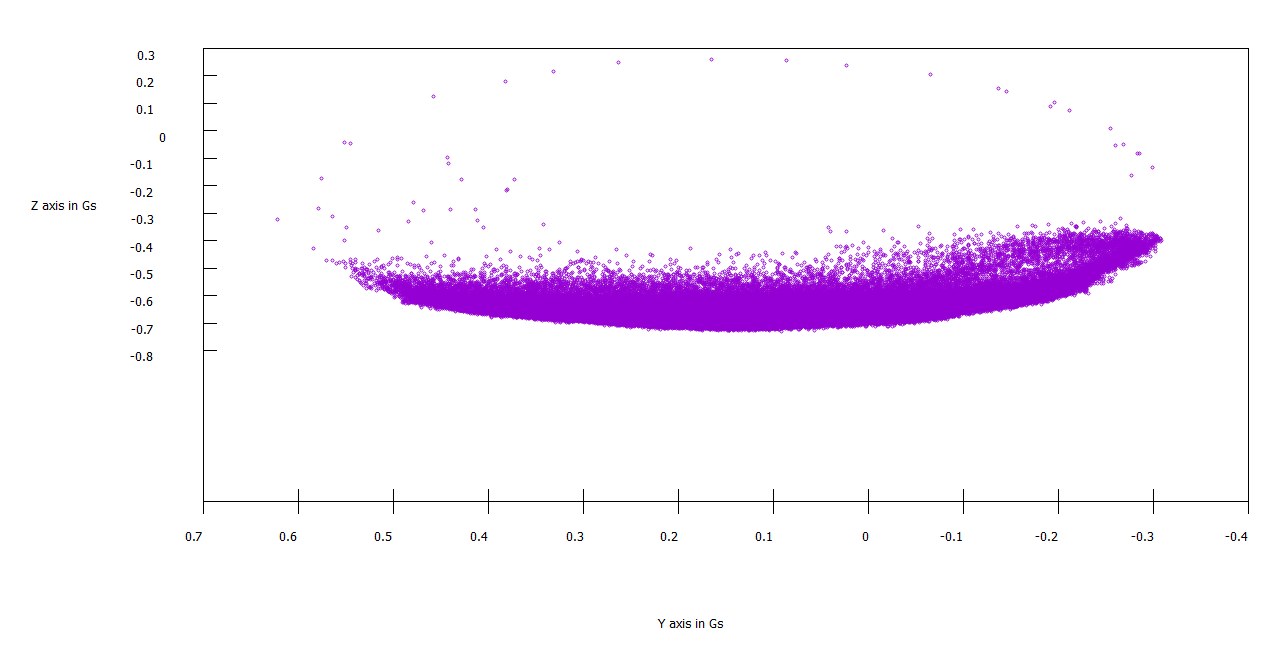
\includegraphics[width=\linewidth]{images/06_conclusion/raw_flight_zy_bowl.png}
    \caption[Plot of the uncalibrated magnetometer data from the junior flight.]{Plot of the uncalibrated magnetometer y- and z-axis data from the junior flight. A bowl shape can clearly be seen in contrast to the spheres used for optimal calibration.}
    \label{fig:conc:flight_bowl}
\end{figure}

To guarantee the best possible calibration, multiple sets of coefficients should be calculated during the different stages of the project to better understand the behaviour of the sensors. After the flight in Kiruna the residuals of all possible calibration coefficient sets, applied to the flight data, can be calculated to determine the parameters with the lowest mean error.